\documentclass{article}
\usepackage{graphicx} %package to manage images
\usepackage[utf8]{inputenc}
\usepackage[a4paper, total={6in, 8in}]{geometry}
\usepackage{xurl}
\usepackage{float}
\title{Relatório 12 \\ Análise completa}
\author{Pedro A. S. O. Neto}
\date{Agosto, 2022}

\begin{document}

\maketitle

\section{Tempo total de fixação - TEA vs Não TEA}

Calcula-se o tempo total de fixação durante cada condição (RJA, IJA), e diagnóstico (TEA vs Não TEA). Hipótese: tempo de fixação difere entre TEA e Não TEA. Essa diferença pode ser maior ou menor entre condições. Método: tempo médio de fixação por indivíduo e condição, comparando entre TEA.

\section{Sample}

Foram analisadas 486 crianças, das quais 20 (4.1\%) receberam diagnóstico de TEA.


\section{Resultados}

\subsection{Comparando entre diagnóstico}

Resultados em segundos.

\begin{table}[ht]
\centering
\begin{tabular}{rlrr}
  \hline
  & TEA & Tempo de fixação & Erro padrão \\
  \hline
  1 & Não & 2.19 & 0.01 \\
  2 & Sim & 1.81 & 0.06 \\
   \hline
\end{tabular}
\end{table}

\begin{figure}[]
\caption{Tempo total de fixação. TEA vs não TEA}
\noindent\makebox[\textwidth]{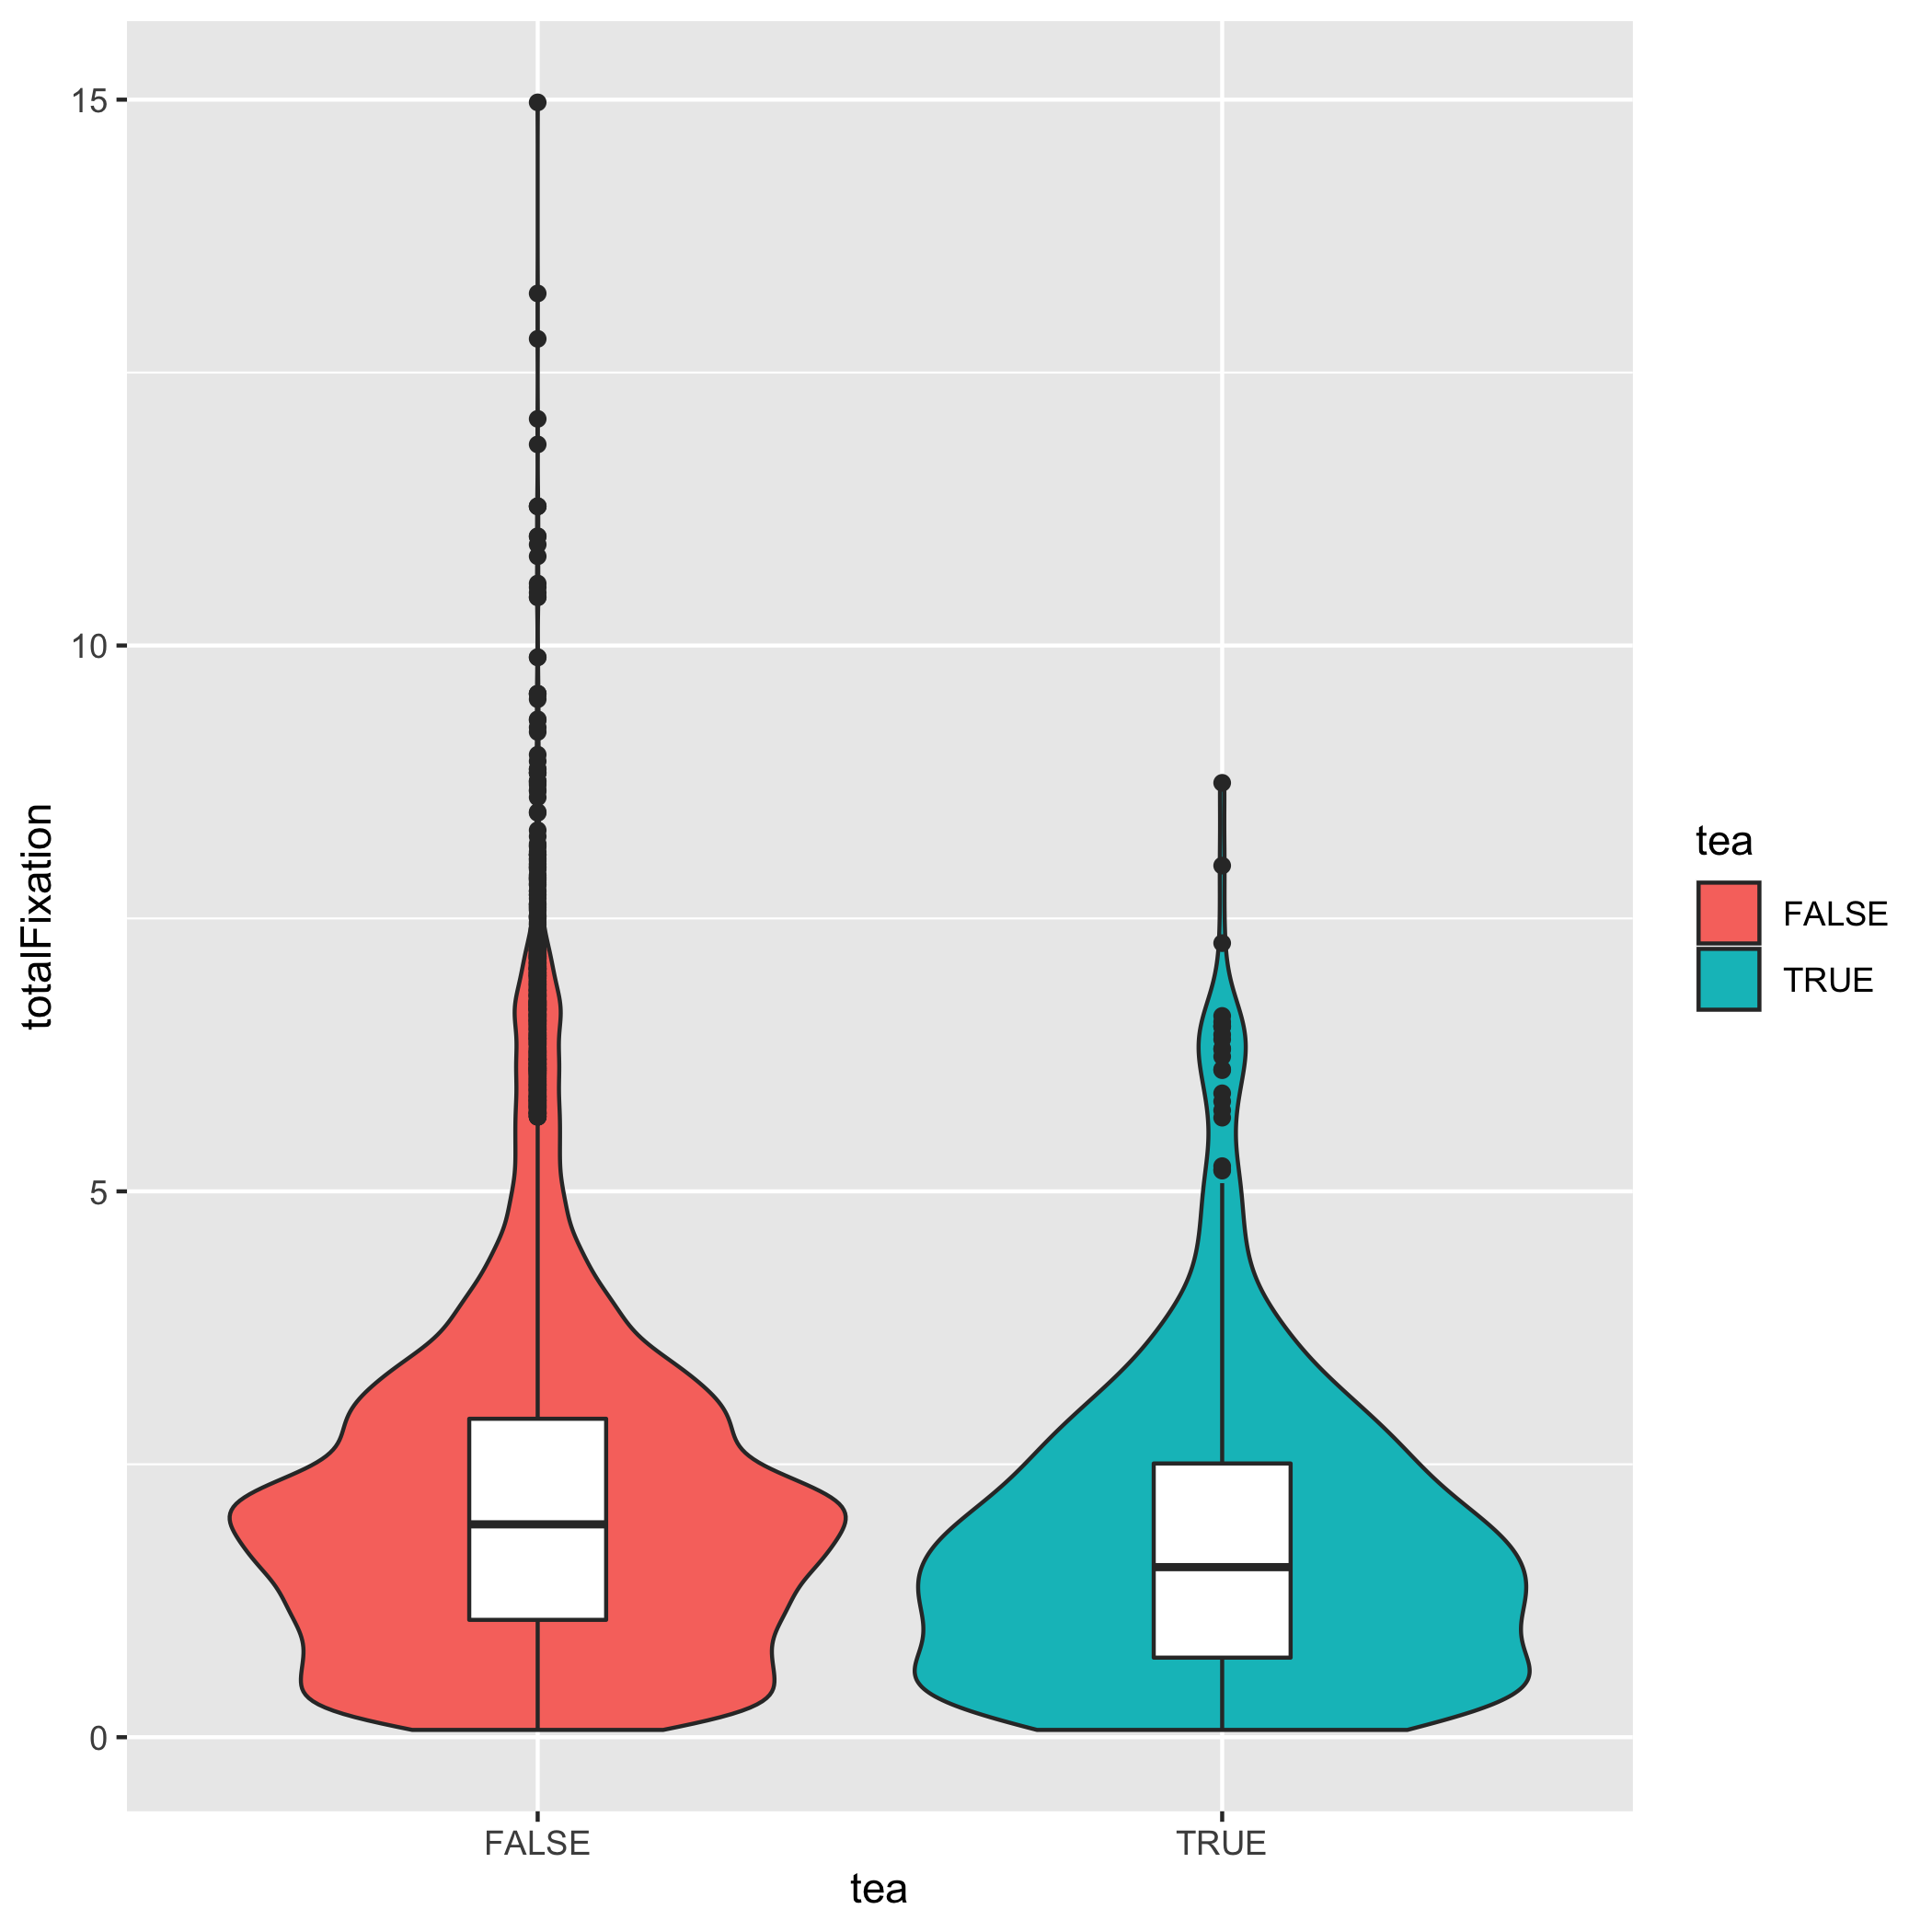
\includegraphics[scale=0.2]{"./boxplot.png"}}
\centering
\end{figure}

\subsection{Comparando entre diagnóstico e condicão}

Condição BL indica (baseline).

\begin{table}[ht]
\centering
\begin{tabular}{rllrr}
  \hline
 & TEA & Condição & Tempo de fixação & Erro padrão \\
  \hline
  1 & Não & BL & 1.84 & 0.01 \\
  2 & Não & IJA & 3.80 & 0.04 \\
  3 & Não & RJA & 2.14 & 0.03 \\
  4 & Sim & BL & 1.56 & 0.05 \\
  5 & Sim & IJA & 3.14 & 0.25 \\
  6 & Sim & RJA & 1.61 & 0.15 \\
  \hline
\end{tabular}
\end{table}

\begin{figure}[]
\caption{Tempo total de fixação. TEA vs não TEA; RJA, IJA, BL}
\noindent\makebox[\textwidth]{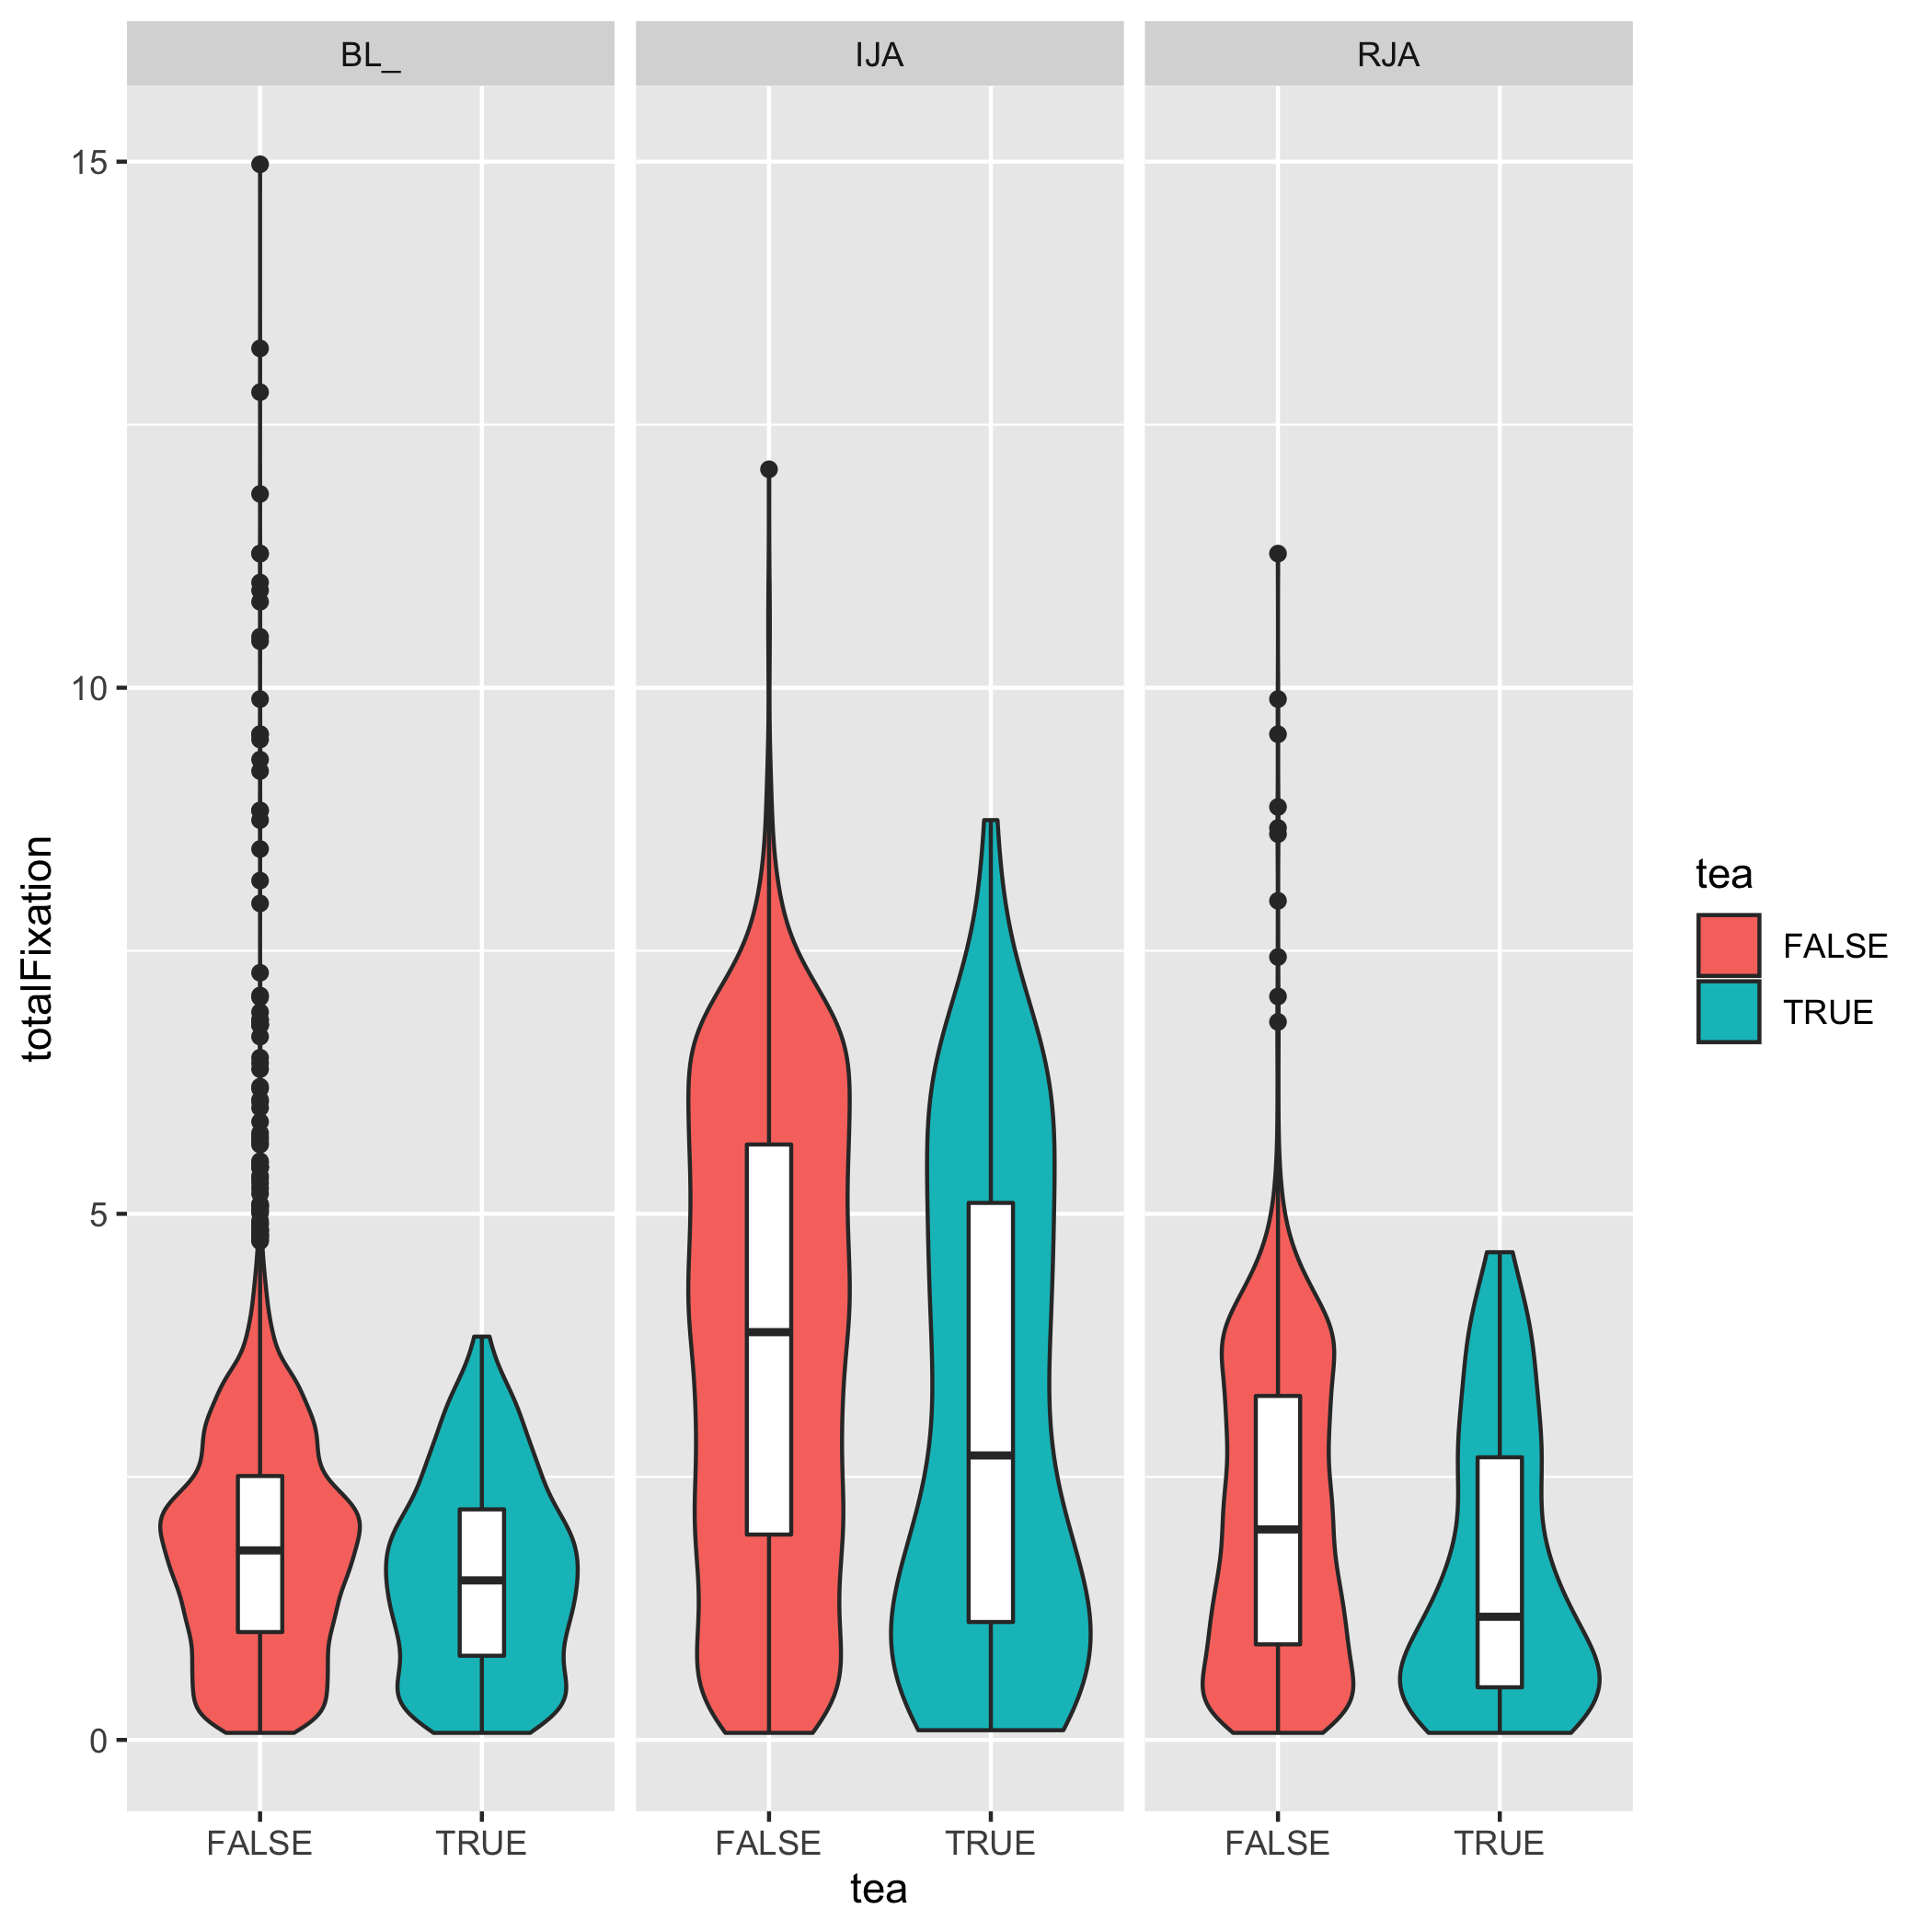
\includegraphics[scale=0.2]{"./boxplot2.png"}}
\centering
\end{figure}

\section{Pupilometria}

Calcula-se o diâmetro de pupila (méia entre pupila direia e esquerda) para cada tipo de diagnóstico, e para cada condição.
Valores indicam o diâmetro da pupila normalizado por criança (z-score). A figura abaixo indica, por exemplo, que crianças sem diagnóstico de TEA têm uma pupila mais dilatada no RJA do que no baseline e no IJA. Crianças com diagnóstico de TEA apresentam dilatação maior no IJA. Porém, o erro padrão é maior, visto que só temos 20 crianças com diagnóstico.

\begin{table}[ht]
\centering
\begin{tabular}{rllrr}
  \hline
 & condition & tea & meanPupil & stder \\
  \hline
  1 & BL\_ & FALSE & -0.01 & 0.01 \\
  2 & BL\_ & TRUE & 0.01 & 0.04 \\
  3 & IJA & FALSE & -0.02 & 0.01 \\
  4 & IJA & TRUE & 0.05 & 0.06 \\
  5 & RJA & FALSE & 0.02 & 0.01 \\
  6 & RJA & TRUE & 0.01 & 0.08 \\
   \hline
\end{tabular}
\end{table}

\begin{figure}[]
\caption{Diâmetro de pupila por condição e diagnóstico.}
\noindent\makebox[\textwidth]{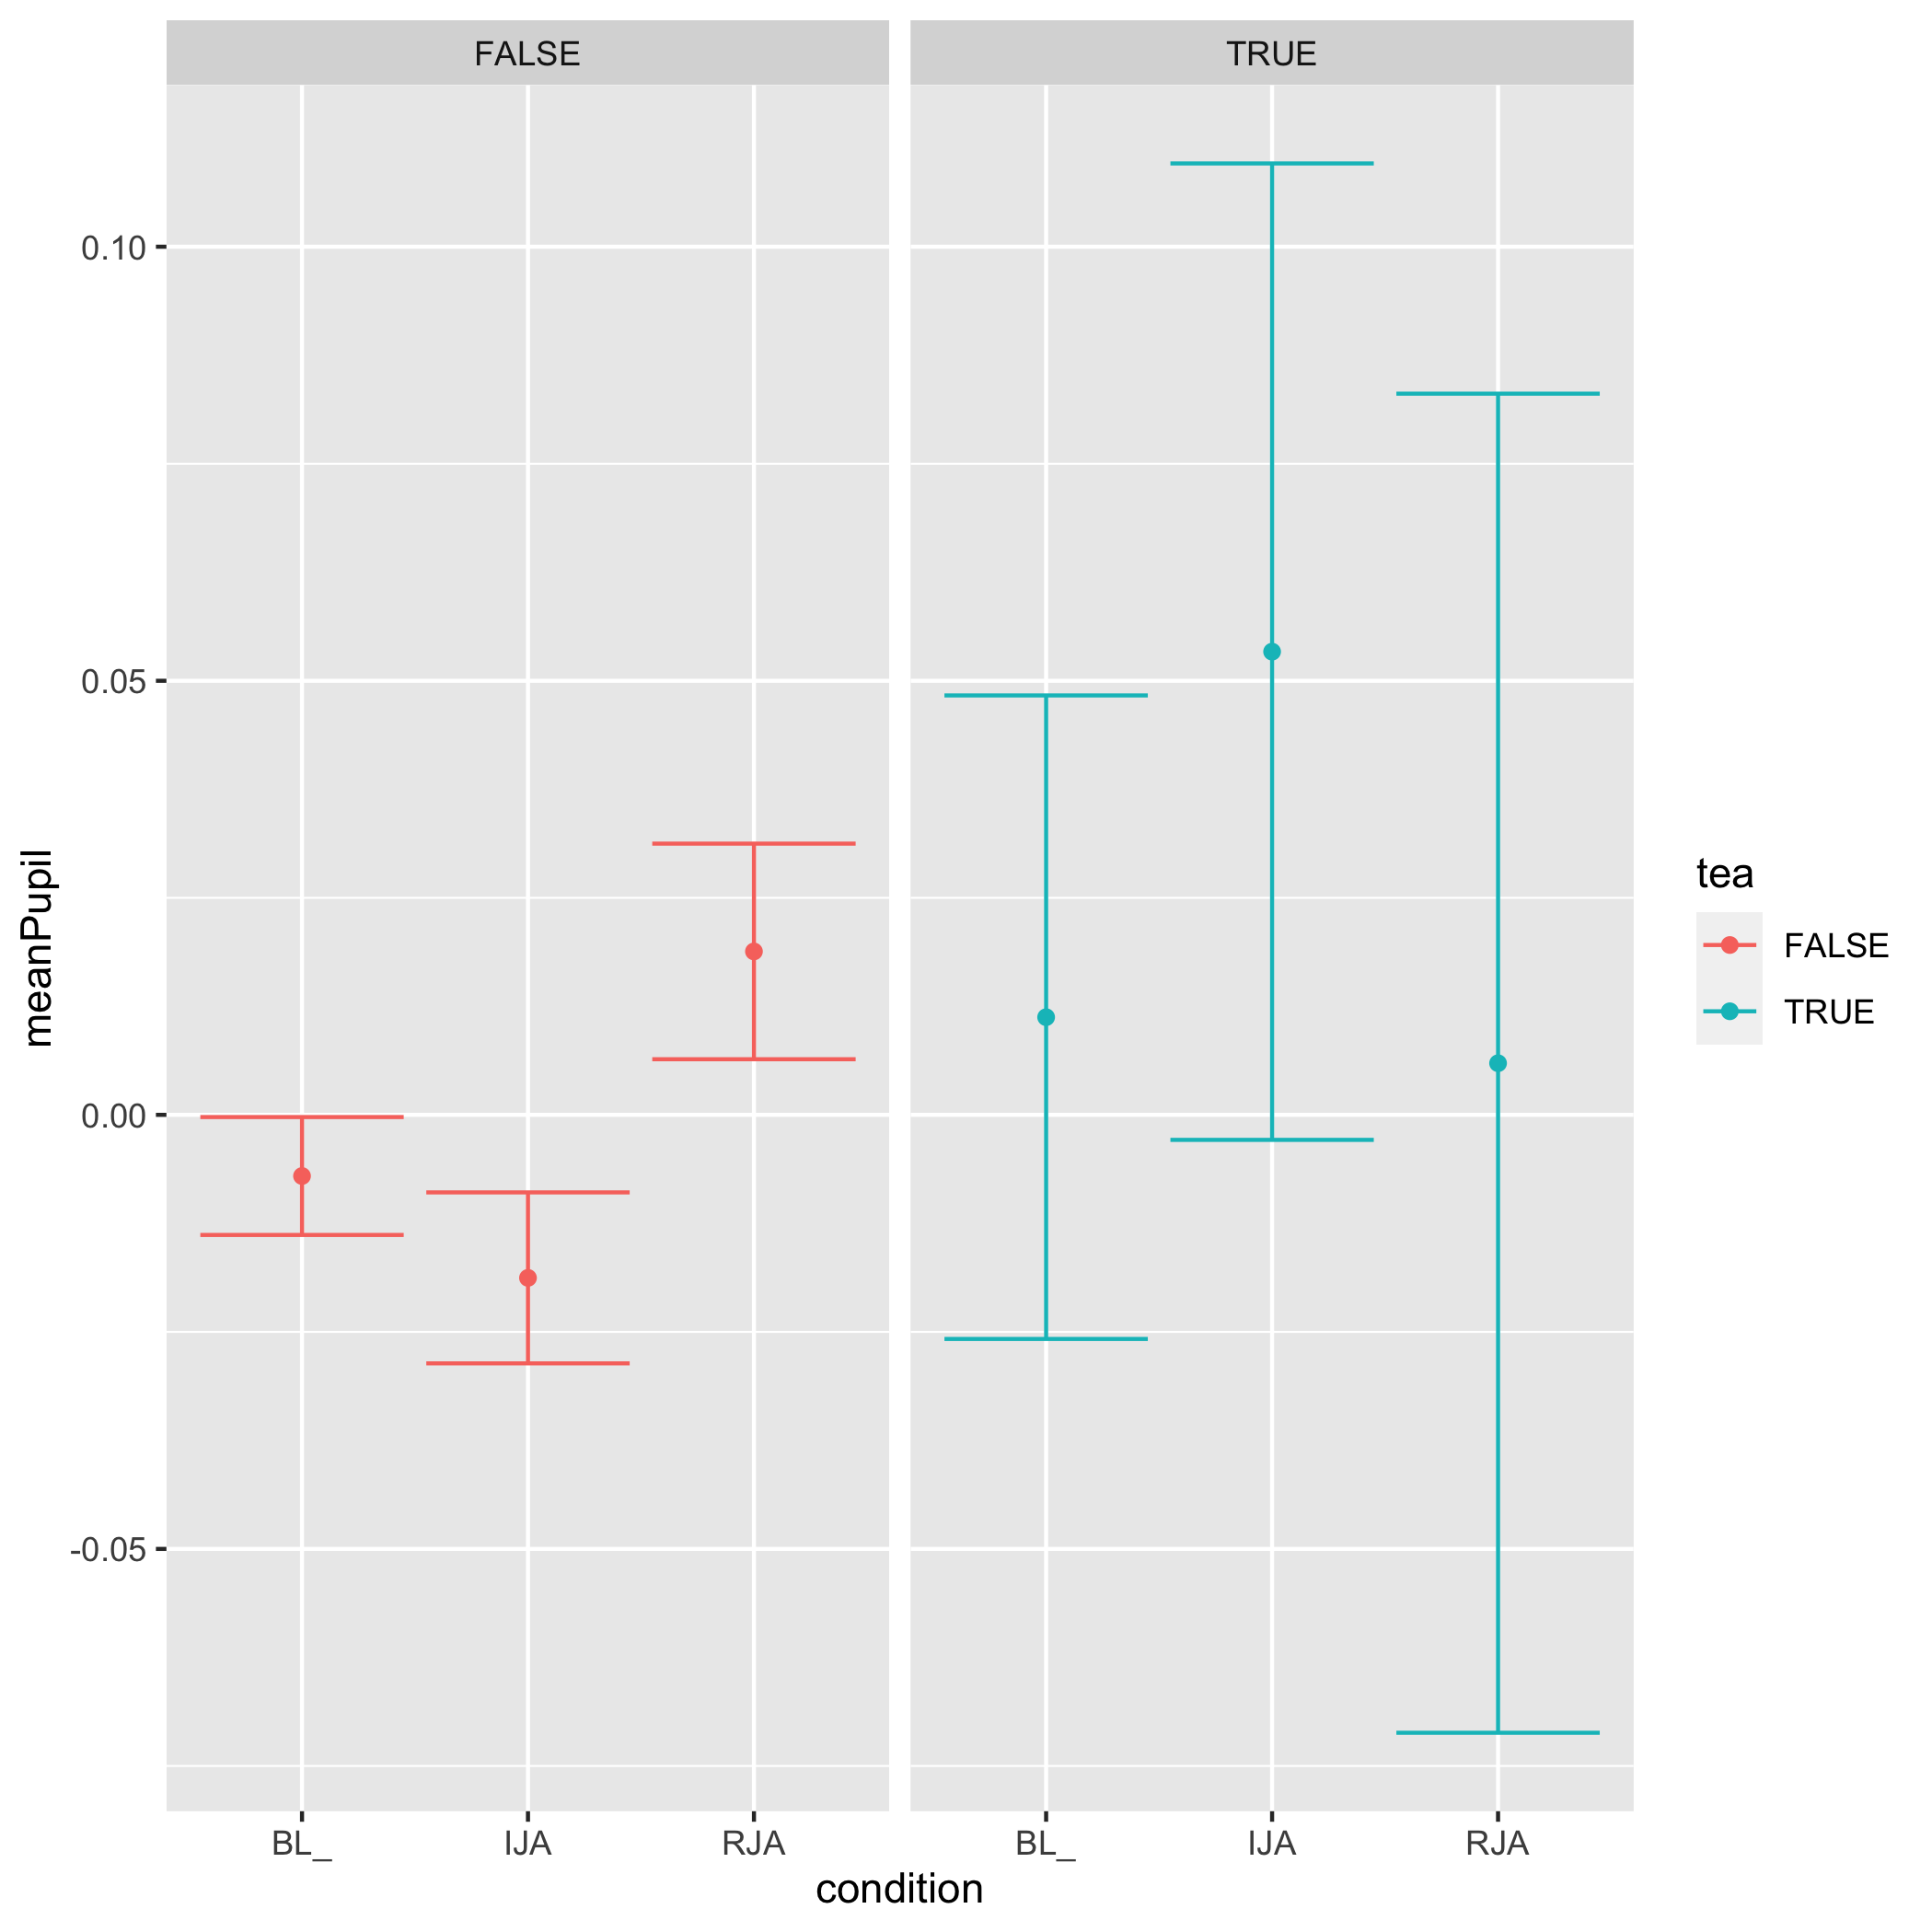
\includegraphics[scale=0.2]{"./pupil.png"}}
\centering
\end{figure}

\section{Alternâncias}

Calcula-se o numero de alternâncias feitas entre Brinquedo Direita e Brinquedo Esquerda para cada condição e diagnóstico. A figura abaixo indica que, na condição IJA, crianças com E sem diagnóstico de TEA, fazem mais alternâncias entre Rosto e Brinquedo da direita quando o foco da tarefa é o brinquedo da direita.

\begin{table}[ht]
\centering
\begin{tabular}{rlllrrrr}
  \hline
 & TEA & Condição & Objeto albo & Rosto-Direita & Rosto-Esquerda & Direita-Rosto & Esquerda-Rosto \\
  \hline
  1 & Não & BL & 1 & 1149.00 & 1131.00 & 825.00 & 822.00 \\
  2 & Não & BL & 2 & 1258.00 & 1400.00 & 916.00 & 1065.00 \\
  3 & Não & IJA & D & 1492.00 & 238.00 & 987.00 & 211.00 \\
  4 & Não & IJA & E & 240.00 & 1504.00 & 239.00 & 1062.00 \\
  5 & Não & RJA & D & 678.00 & 265.00 & 441.00 & 189.00 \\
  6 & Não & RJA & E & 282.00 & 721.00 & 209.00 & 462.00 \\
  7 & Sim & BL & 1 & 37.00 & 42.00 & 27.00 & 27.00 \\
  8 & Sim & BL & 2 & 37.00 & 44.00 & 25.00 & 31.00 \\
  9 & Sim & IJA & D & 41.00 & 10.00 & 28.00 & 7.00 \\
  10 & Sim & IJA & E & 4.00 & 46.00 & 4.00 & 35.00 \\
  11 & Sim & RJA & D & 10.00 & 10.00 & 6.00 & 4.00 \\
  12 & Sim & RJA & E & 7.00 & 18.00 & 7.00 & 13.00 \\
   \hline
\end{tabular}
\end{table}


\begin{figure}[]
\caption{IJA - Número de alternâncias entre objetos (Rosto, brinquedo direita e brinquedo esquerda). Eixo X indica o foco da tarefa (Brinquedo direita ou esquerda). Eixo Y indica a contagem total de alternâncias. False/True indica se diagnóstico TEA é Sim ou Não.}
\noindent\makebox[\textwidth]{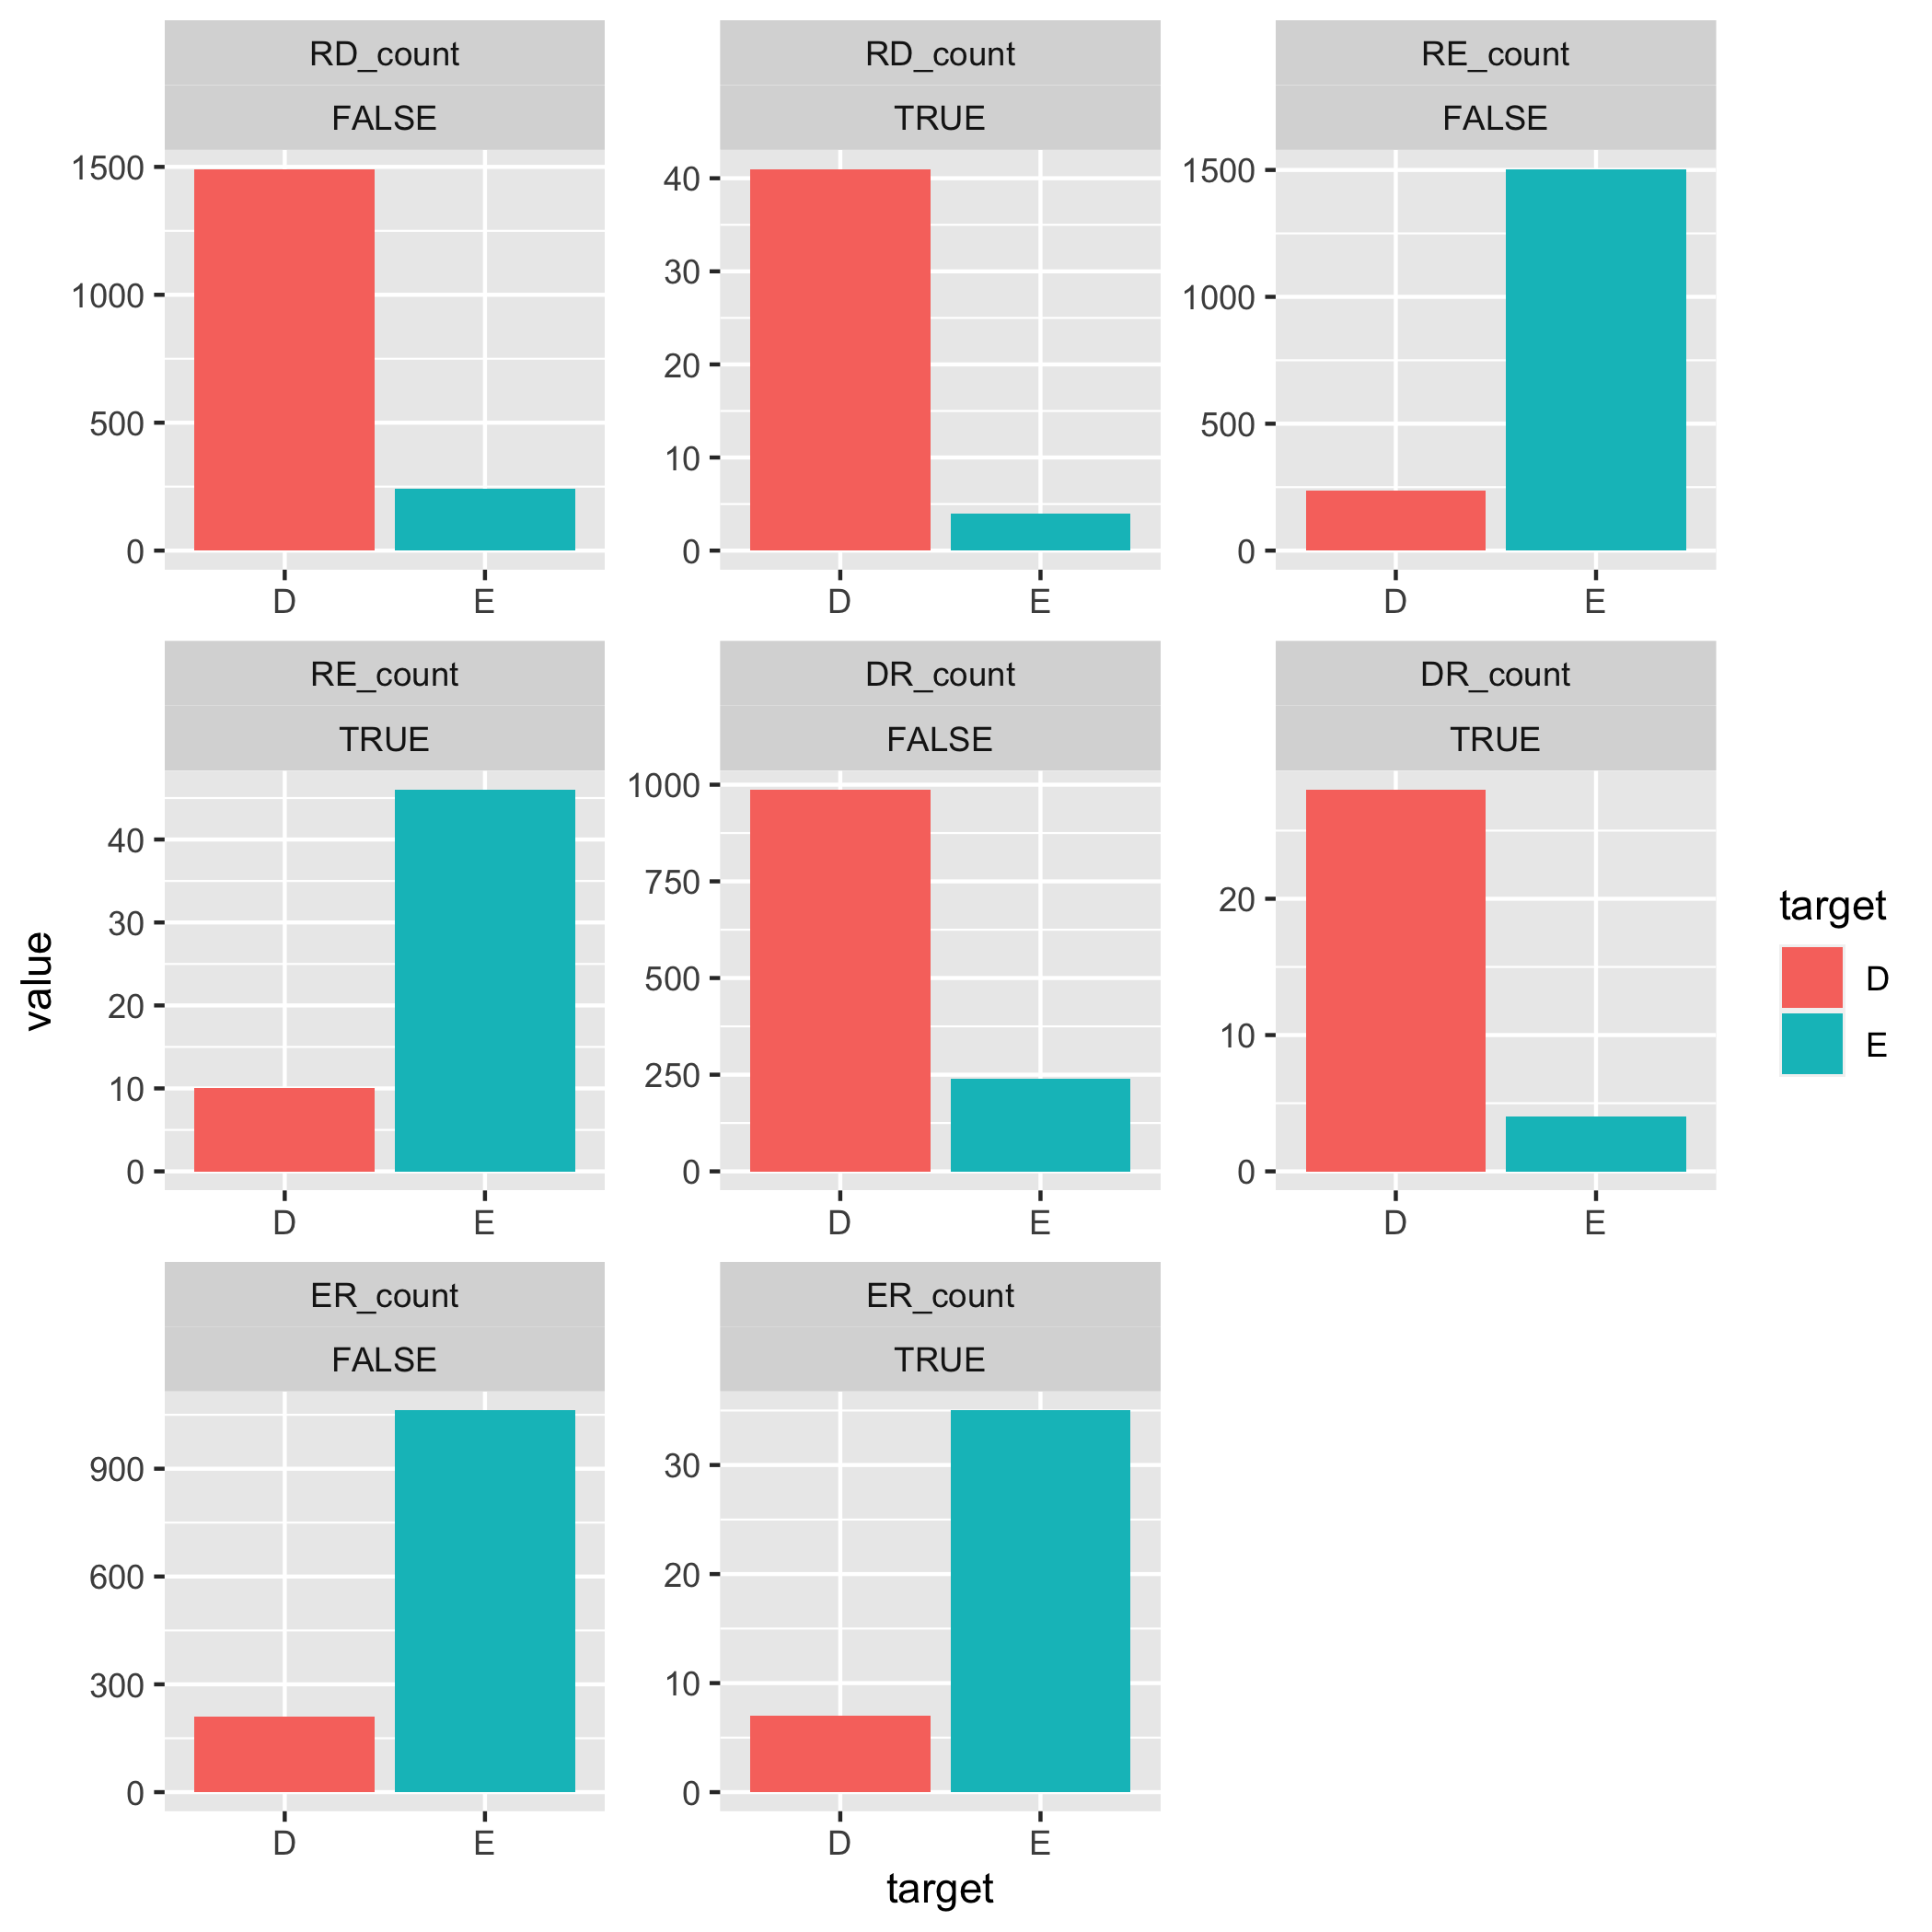
\includegraphics[scale=0.2]{"./alternanciaIJA.png"}}
\centering
\end{figure}

\begin{figure}[]
\caption{RJA - Número de alternâncias entre objetos (Rosto, brinquedo direita e brinquedo esquerda). Eixo X indica o foco da tarefa (Brinquedo direita ou esquerda). Eixo Y indica a contagem total de alternâncias. False/True indica se diagnóstico TEA é Sim ou Não.}
\noindent\makebox[\textwidth]{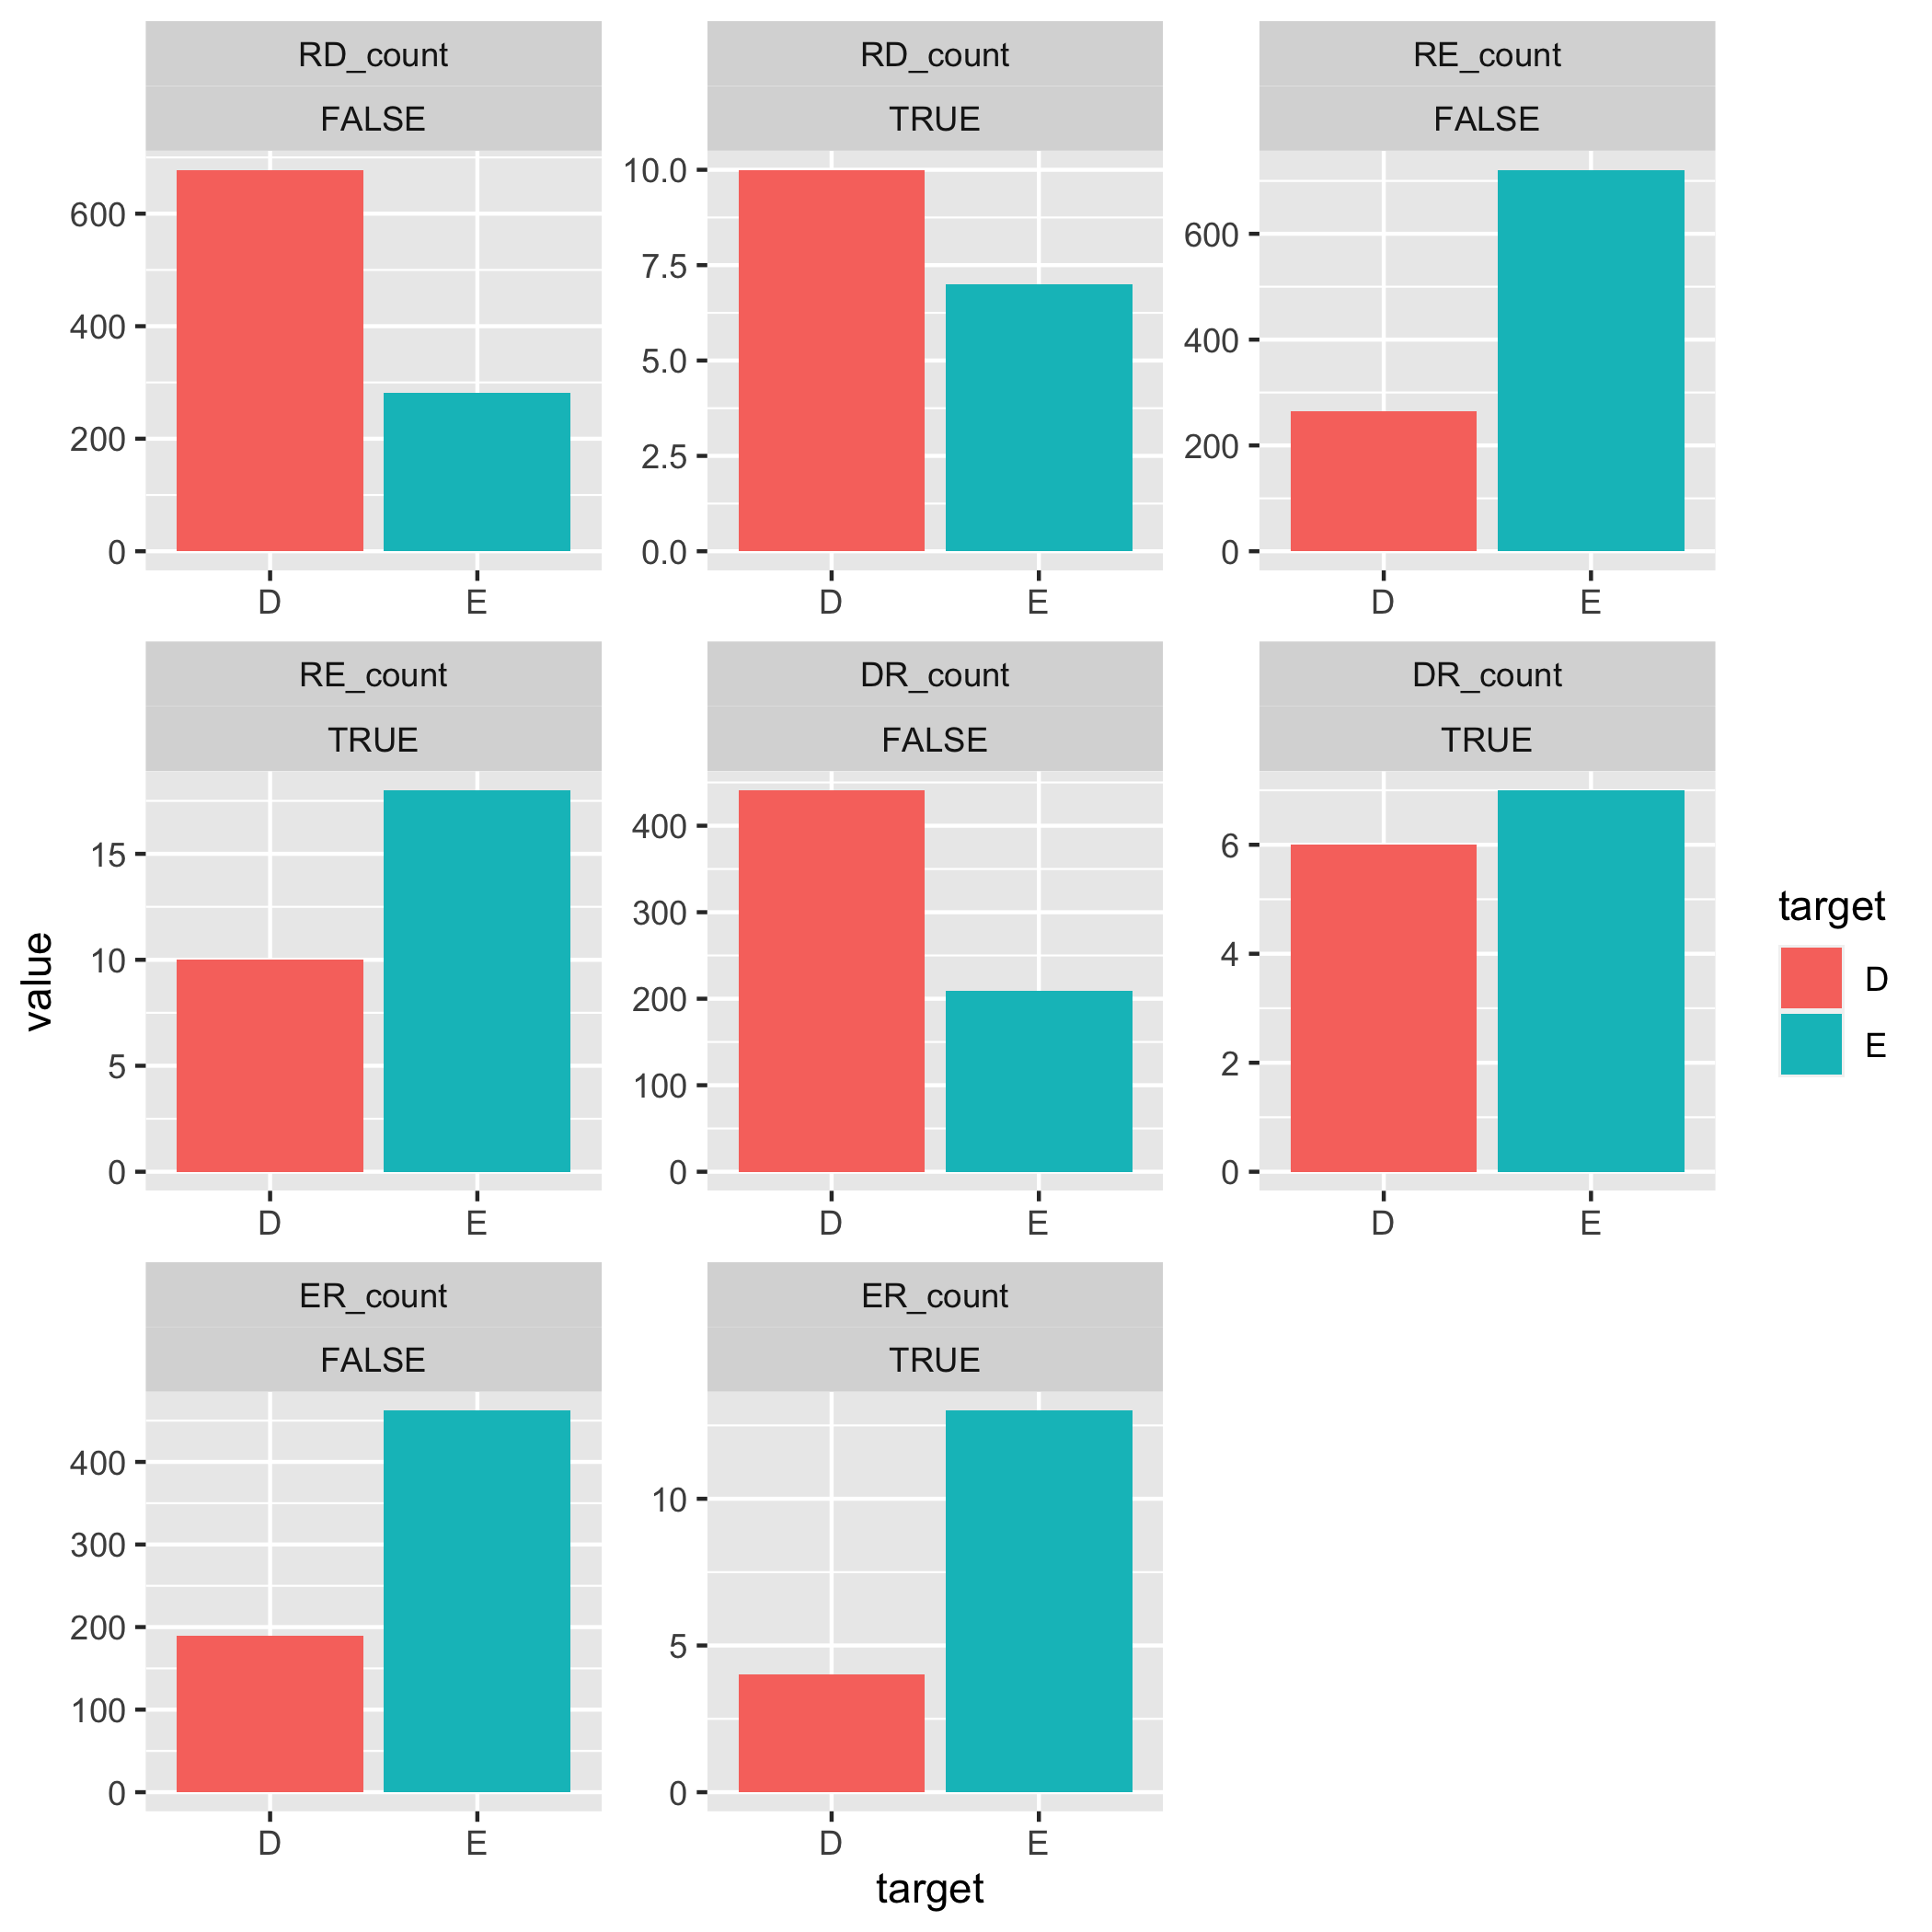
\includegraphics[scale=0.2]{"./alternanciaRJA.png"}}
\centering
\end{figure}



\end{document}
